\documentclass{InsightArticle}

\usepackage[dvips]{graphicx}
\usepackage{float}
\usepackage{subfigure}

\usepackage[dvips,
bookmarks,
bookmarksopen,
backref,
colorlinks,linkcolor={blue},citecolor={blue},urlcolor={blue},
]{hyperref}

\title{Boost's Douglas-Peucker Contour Simplification Wrapper for ITK and VTK}

% 
% NOTE: This is the last number of the "handle" URL that 
% The Insight Journal assigns to your paper as part of the
% submission process. Please replace the number "1338" with
% the actual handle number that you get assigned.
%
\newcommand{\IJhandlerIDnumber}{3302}

% Increment the release number whenever significant changes are made.
% The author and/or editor can define 'significant' however they like.
\release{0.00}

% At minimum, give your name and an email address.  You can include a
% snail-mail address if you like.

\author{David Doria}
\authoraddress{Rensselaer Polytechnic Institute}


\begin{document}

\IJhandlefooter{\IJhandlerIDnumber}


\ifpdf
\else
   %
   % Commands for including Graphics when using latex
   % 
   \DeclareGraphicsExtensions{.eps,.jpg,.gif,.tiff,.bmp,.png}
   \DeclareGraphicsRule{.jpg}{eps}{.jpg.bb}{`convert #1 eps:-}
   \DeclareGraphicsRule{.gif}{eps}{.gif.bb}{`convert #1 eps:-}
   \DeclareGraphicsRule{.tiff}{eps}{.tiff.bb}{`convert #1 eps:-}
   \DeclareGraphicsRule{.bmp}{eps}{.bmp.bb}{`convert #1 eps:-}
   \DeclareGraphicsRule{.png}{eps}{.png.bb}{`convert #1 eps:-}
\fi


\maketitle


\ifhtml
\chapter*{Front Matter\label{front}}
\fi

\begin{abstract}
\noindent

This document presents wrappers (ITK and VTK) of the Boost Geometry Library algorithm to find a low edge-count approximation of a complex, discrete, 2D contour. The contour can be open or closed.

The code is available here:
\verb|https://github.com/daviddoria/DouglasPeuckerPolylineSimplification|

\end{abstract}

\IJhandlenote{\IJhandlerIDnumber}

\tableofcontents
%%%%%%%%%%%%%%%%%%%%
\section{Introduction}
This document presents ITK and VTK wrappers to an algorithm to find a low edge-count approximation of a complex, discrete, 2D  contour. Our goal is to represent the outline of an object in a simple fashion.

%%%%%%%%%%%%%%%%%%%%
\section{Algorithm}
\label{sec:Algorithm}
The algorithm is explained very well here:
\verb|http://www.softsurfer.com/Archive/algorithm_0205/algorithm_0205.htm|

We include excerpts below to make this document self contained. The algorithm consists of two steps, vertex reduction and then Douglas-Peucker simplification.

\subsection{Vertex Reduction}
``Vertex reduction is the brute-force algorithm for polyline simplification.  For this algorithm, a polyline vertex is discarded when its distance from a prior initial vertex is less than some minimum tolerance $\epsilon > 0$.   Specifically,  after fixing an initial vertex $V_0$, successive vertices $V_i$ are tested and rejected if they are less than $\epsilon$ away from $V_0$. But, when a vertex is found that is further away than $\epsilon$, then it is accepted as part of the new simplified polyline, and it also becomes the new initial vertex for further simplification of the polyline.''

\subsection{Douglas-Peucker Simplification}
``Whereas vertex reduction uses closeness of vertices as a rejection criterion, the Douglas-Peucker (DP) algorithm uses the closeness of a vertex to an edge segment.  This algorithm works from the top down by starting with a crude initial guess at a simplified polyline, namely the single edge joining the first and last vertices of the polyline.   Then the remaining vertices are tested for closeness to that edge.  If there are vertices further than a specified tolerance, $\epsilon > 0$, away from the edge, then the vertex furthest from it is added the simplification.  This creates a new guess for the simplified polyline.  Using recursion, this process continues for each edge of the current guess until all vertices of the original polyline are within tolerance of the simplification.''

%%%%%%%%%%%%%%%%%%%%
\section{Parameters}
The only parameter to the algorithm is the ``approximation tolerance'', which is a distance value that determines how simplified the contour becomes. The larger the tolerance, the more simplification will take place.

%%%%%%%%%%%%%%%%%%%%
\section{VTK Wrapper}
The VTK representation of a contour is a \verb|vtkPolyData| whose CellArray contains a list of ordered vtkLine objects. We therefore provide a wrapper with signature:

\begin{verbatim}
void SimplifyPolyline( vtkPolyData* input, float tolerance, vtkPolyData* output)
\end{verbatim}

\subsection{ITK Wrapper}
The ITK representation of a contour is a \verb|itk::PolyLineParametricPath< 2 >|. We therefore provide a wrapper with signature:

\begin{verbatim}
void SimplifyPolyline( itk::PolyLineParametricPath< 2 >::Pointer input, 
                       float tolerance, 
                       itk::PolyLineParametricPath< 2 >::Pointer output);
\end{verbatim}

%%%%%%%%%%%%%%%%%%%%
\section{Demonstration}

A typical case of the simplification of a contour is shown in Figure \ref{fig:Demo}.

\begin{figure}[H]
  \centering
  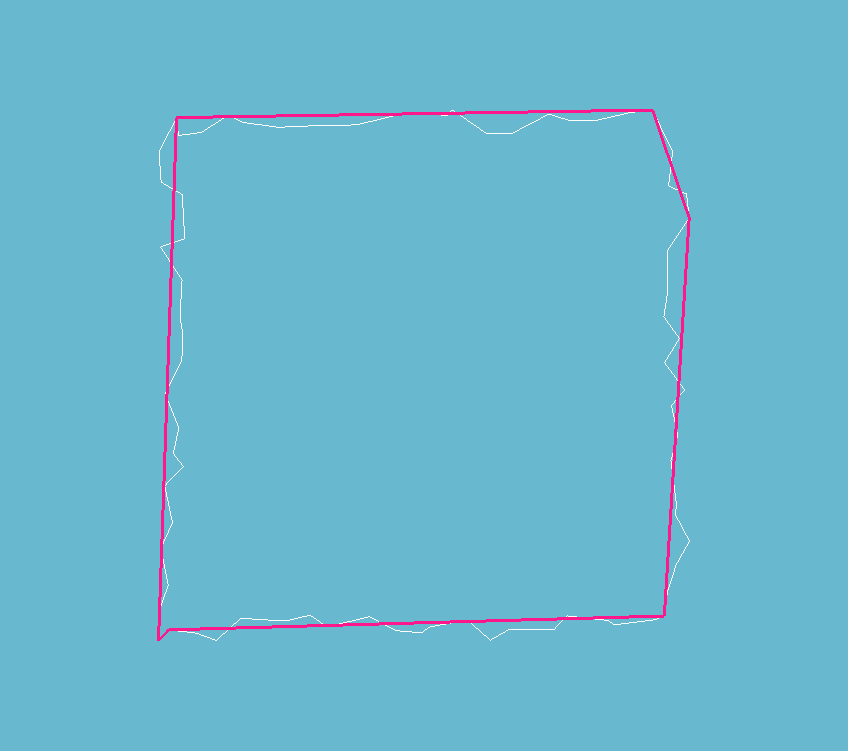
\includegraphics[width=0.3\linewidth]{images/demo}
  \caption{A demonstration of the simplification algorithm. The original contour is shown in white, where the simplified contour (tolerance = 1.0) is shown in red.}
  \label{fig:Demo}
\end{figure}




\end{document}
